%
% paper title
% section title
%

\documentclass[ master_reopn ]{subfiles}
\begin{document}         

\section{Linear rewriting} \label{sec_linear}

\todo{X shd b topos for intrchng}
\todo{remind linear meaning}

\begin{df} \label{df_linrewrite-obcat}
	From a category $ \A $ with pullbacks, construct a category $ \MM_0 \coloneqq \core (\Span (\A)) $ whose objects are those of $ \A $ and arrows are spans in $ \A $ with invertible legs.  	
\end{df}

\begin{df} \label{df_linrewrite-arrcat}
		Consider a functor $ L \from \A \to \X $ from a category $ \A $ with pullbacks to a topos $ \X $. Denote by $ \MM_1 $ the category whose objects are $ L $-structured cospans
			\edit{open objects?}
		and arrows are isomorphism classes of spans of $ L $-structured cospans
	\[
	\diagram{diag_linrewrite-2cell}
	\]
	where the arrows marked ``$ \rightarrowtail $'' are monic. Such an isomorphism class is an invertible $ \X $-arrow $ y \to y' $ that fits into the commuting pasting diagram obtained by identifying the outer squares of the spans of $ L $-structured cospans
	\[
	\diagram{diag_linrewrite_iso-sp-csp}
	\]
\end{df}

\begin{lem} \label{df_mon-rewrite-dble-cat}
	Consider a functor $ L \from \A \to \X $ from a category $ \A $ with pullbacks to a topos $ \X $.  Denote by $ \MMonRewrite_{L} $ the double category with $ \A $-objects as 0-cells, spans in $ \A $ with invertible legs as vertical 1-cells, $ L $-structured cospans as horizontal 1-cells, and commuting diagrams in $ \X $ of form	
	\[
	\diagram{diag_linrewrite-2cell}
	\]
	
	In particular, $ \MMonRewrite_{L} $ consists of the object category $ \MM_0 $; arrow category $ \MM_1 $; unit functor $ U \from \MM_0 \to \MM_1 $ defined by
	\[
	\diagram{diag_linrewrite-unit-functor}
	\]
	source and target functors $ S , T \from \MM_1 \to \MM_0 $ respectively defined by
	\[
	\diagram{diag_linrewrite-source-functor}
	\quad \text{and} \quad
	\diagram{diag_linrewrite-target-functor}
	\]
	and composition functor $ \odot \from \MM_1 \times_{\MM_0} \MM_1 \to \MM_1 $ defined by
	\[
	\diagram{diag_linrewrite-composition-functor}
	\]
	which uses pushouts in $ \X $ and their universal properties. 
\end{lem}
\begin{proof}
	\edit{say why compositie gives monics.}
\end{proof}

\begin{thm} \label{thm_mon-rewrite-isofibrant}
	The double category $ \MMonRewrite{L} $ is isofibrant.
\end{thm}
\begin{proof}
	A companion for the vertical 1-cell $ a \xto{f} b \xgets{g} c $ is the same as used in Theorem \ref{thm_rewrite-isofibrant}.  
	
	\edit{remains to show the equations hold}
\end{proof}

\begin{thm} \label{thm_mon-rewrite-dble-cat-smc}
	Let $ (\A, \otimes_{ \A }, I_{ \A }) $ and $ (\X, \otimes_{\X}, I_{\X}) $ be symmetric monoidal categories where $ \A $ has pullbacks and $ \X $ is a topos. Let $ L \from (\A, \otimes_{ \A }, I_{ \A }) \to (\X, \otimes_{\X}, I_{\X}) $ be a pullback preserving functor. Then $ (\MMonRewrite{L} , \otimes , I) $ is a symmetric monoidal double category with $ \otimes $ defined by
	\[
	\left( L a \to x \gets L b \right) \otimes
	\left( L c \to y \gets L d	\right) \coloneqq
	L (a \otimes_{\A} c) \to 
	x \otimes_{\X} y \gets L (b \otimes_{\A} d)
	\]
	and $ I $ by
	\[
	I \coloneqq ( L I_{\A} \to I_{\X} \gets L I_{\X} ).
	\]
\end{thm}

\begin{thm} \label{thm_mon-rewrite-cat-compact-closed}
	Let $ (\A, \otimes_{ \A }, I_{ \A }) $ and $ (\X, \otimes_{\X}, I_{\X}) $ be symmetric monoidal categories where $ \A $ has pullbacks and $ \X $ is a topos. Let $ L \from (\A, \otimes_{ \A }, I_{ \A }) \to (\X, \otimes_{\X}) $ be an adjunction where $ L $ preserves pullbacks.
	
	The horizontal edge bicategory $ \MonRewrite{L} \coloneqq  \mathcal{H} \left( \MMonRewrite{L} \right) $ in the sense of Shulman is symmetric monoidal.  Moreover, if the monoidal products $ \otimes_{\A} $ and $ \otimes_{\X} $ are coproducts, then the symmetric monoidal bicategory $ \MonRewrite{L} $ is compact closed.
\end{thm}


\begin{thm}
	Suppose each element from a grammar $ \Gamma $ in $ \Cospan_{L} $ is of the form 
	\[
	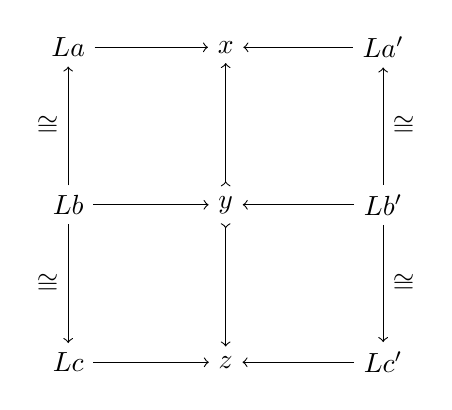
\begin{tikzpicture}
	\node (a) at (-1,1) {$ L a $};
	\node (x) at (1,1) {$ x $};
	\node (a') at (3,1) {$ L a' $};
	\node (b) at (-1,-1) {$ L b $};
	\node (y) at (1,-1) {$ y $};
	\node (b') at (3,-1) {$ L b' $};
	\node (c) at (-1,-3) {$ L c $};
	\node (z) at (1,-3) {$ z $};
	\node (c') at (3,-3) {$ L c' $};
	%
	\draw [->] (a) to (x);
	\draw [->] (a') to (x);
	\draw [->] (b) to (y);
	\draw [->] (b') to (y);
	\draw [->] (c) to (z);
	\draw [->] (c') to (z);
	\draw [->] (b) to node [left] {$ \cong $} (a);
	\draw [->] (b) to node [left] {$ \cong $} (c);
	\draw [>->] (y) to (x);
	\draw [>->] (y) to (z);
	\draw [->] (b') to node [right] {$ \cong $} (a');
	\draw [->] (b') to node [right] {$ \cong $} (c');
	\end{tikzpicture}
	\]
	then $ \Gamma $ generates a sub-double category $ \langle \langle \Gamma \rangle \rangle $ of $ \MMonRewrite_{L} $.  The recipe is get the language $ \mathcal{L}(\Gamma)  \subseteq \Span {(\Cospan_{L})} $. Form the category as described in Definition \ref{df:ArrCatMonRwrt} from $ \mathcal{L}(\Gamma) $. Pair this, as an arrow category, with the object category $ \core (\Span_{\A}) $.
\end{thm}

\begin{thm}
	Same as above with monics thrown in.
\end{thm}

\end{document}